\chapter{Návrh analýzy}
\label{possible-analysis-strategies}

% TODO uistit sa, ze \ref-s naozaj obsahujú informácie, na ktoré sa odkazujem

V tejto kapitole popisujem návrh na vypracovanie analýzy nasadenia a využívania technológie NEL.

\subsubsection{Cieľ a rozsah}

Cieľom práce je analyzovať nasadenie technológie NEL na webe. 
Vďaka dostupným zdrojom dát popisovaných v kapitole \ref{data-sources-available-for-research} je možné skúmať stav využívania NEL:
\begin{enumerate}
    \item v histórií prehliadania webu zaznamenanej v dátach poskytovaných projektom HTTP Archive,
    \item v súčasnosti použitím automatizovaného webového prehliadania -- web crawling.
\end{enumerate}

Na základe konzultácie s vedúcim tejto práce, pánom Polčákom, som sa rozhodol analýzu zhotoviť pre čo 
najrozsiahlejšie obdobie.
Zámerom je pokúsiť sa pokryť celé obdobie, za ktoré sa NEL doteraz používalo, no závisí na zdrojoch použitých pre analýzu, či budú všetky potrebné dáta dostupné.
Ako počiatočný dátum môžem zvoliť 25. september 2018, kedy autori tejto technológie publikovali jej špecifikáciu (viď sekciu \ref{network-error-logging}).
Od tohto počiatočného dátumu chcem zhotoviť prieskum až po dátum obhajoby tejto práce -- máj 2024.

\subsubsection{Existujúca analýza}

Taktiež som sa v rámci konzultácií zameral na získanie cenných informácií a poučení z existujúcej analýzy z roku 2023,
ktorú zhotovil pán Polčák spolu s jeho kolegom, pánom Jeřábkom \cite{nel-http-archive}.
Je zameraná na získanie metrík ako celkové využívanie NEL na množine skúmaných domén (viď obrázok \ref{fig:polcak-analysis}), aké NEL kolektory dané domény používajú a v akých konfiguráciách sa nasadené NEL vyskytuje.
Časové obdobie, za ktoré bola analýza zhotovená, tvorili februárové mesiace každého roku od 2018 do 2023. 
Za toto obdobie sa im podarilo zistiť, že počiatočné využitie NEL bolo 0\% a do februára roku 2023 stúplo na 11.73\% skúmaných domén.
Toto percento predstavuje z celkového počtu skúmaných domén 2,247,233 jedinečných domén.

\begin{figure}[!htb]
\begin{center}
    % 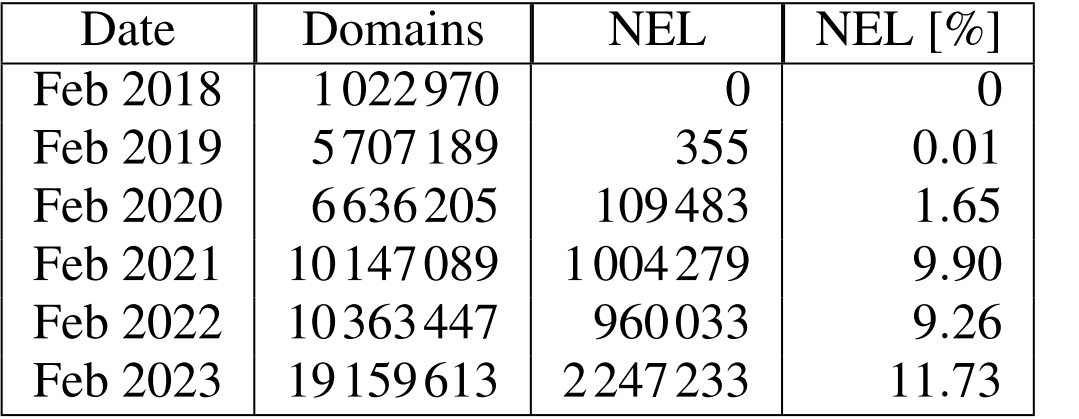
\includegraphics[width=0.5\linewidth]{obrazky-figures/polcak-analysis.png}
    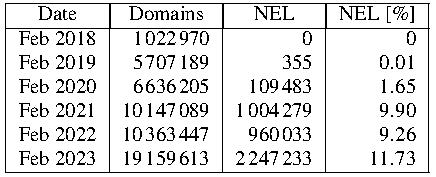
\includegraphics[width=0.55\linewidth]{obrazky-figures/polcak-analysis-hd.pdf}
    \caption{\centering Využitie NEL na skúmaných doménach v analýze vypracovanej vo vedeckom článku Ing. Libora Polčáka Ph.D. a Ing. Kamila Jeřábka \cite{nel-http-archive}.}
    \label{fig:polcak-analysis}
\end{center}
\end{figure}

\pagebreak

Zistil som, že ako zdroj dát bol použitý HTTP Archive, ktorým sa zaoberá aj moja práca.
Je však dôležité poznamenať, že predošlá analýza bola vypracovaná iba za pomoci využitia 
práve jedného zdroja dostupného na každej skúmanej doméne.
Keďže bol v rámci práce použitý projekt HTTP Archive ako zdroj dát, k tomuto rozhodnutiu obmedziť sa mohlo viesť to, 
že ním využívaná služba BigQuery je spoplatnená (viď sekciu \ref{big-query}). 
Je pravdepodobné, že autori nemali prostriedky pre financovanie spracovania takého veľkého objemu dát, 
ktorý predstavuje skúmané obdobie šiestich rokov (od 2018 do 2023).
Vo svojej práci usúdili, že vzhľadom na túto limitáciu je nutné vypracovať podrobnejšiu analýzu, 
doplnenú o dáta získané alternatívnym spôsobom \cite{nel-http-archive}.
Práve z toho dôvodu som počiatočne usúdil, že je nutné v mojej analýze okrem použitia HTTP Archive navrhnúť 
aj iný spôsob skúmania stavu využitia technológie NEL.

\subsubsection{Prieskum možností pre vylepšenia}

Preskúmal som spôsob, ktorý vo vyššie uvedenej práci použili na získavanie HTTP Archive dát.
Bol použitý nástroj pre sťahovanie dát z Google Cloud BigQuery, ktorý naprogramoval pán 
Jeřábek\footnote{\href{https://github.com/kjerabek/nel-http-archive-analysis}{https://github.com/kjerabek/nel-http-archive-analysis}}.
Počas testovania tohto nástroja som zistil, že je možné vylepšiť ho tak, aby som odstránil predošlú, v skutočnosti iba myslenú limitáciu s nedostatkom dát kvôli financiám.
Postupným skúšaním používania a úprav príkazu GoogleSQL použitého v spomínanom nástroji na extrahovanie dát som prišiel na skutočnosť, že BigQuery
si nárokuje poplatky nie za sťahovanie, ale za čítanie dát z jednotlivých stĺpcov svojich tabuliek.
To pre mňa znamenalo, že nebudem platiť za objem dát, ktoré stiahnem, ale za objem dát, ktoré pri spustení príkazu GoogleSQL bude musieť služba prečítať.
Prišiel som teda na to, že rozhodnutie obmedziť sa na jeden zdroj pre každú skúmanú doménu v predošlej analýze nezaručilo nižšiu spotrebu financií.
Tým pádom sa pre mňa otvorila možnosť naplno využiť HTTP Archive dáta úpravou spomínaného príkazu GoogleSQL, pričom by som na to potreboval rovnakú sumu peňazí.
Táto úprava spočívala v odstránení filtrov z tohto príkazu, ktoré jeho výsledné dáta limitovali na jeden zdroj pre každú doménu.

Google Cloud ako platforma pre BigQuery v dobe vypracovania mojej práce ponúkala novo zaregistrovaným účtom zadarmo skúšobný
kredit 300\$. 
Podľa BigQuery cenníka viem, že 1 terabajt prečítaných dát stojí 6.25\$.
To by znamenalo, že s využitím ponúkaného kreditu mám dostupnú kapacitu 48 terabajtov, 
pričom s každým uplynulým mesiacom získam ďalší terabajt naviac (viď ceny služby GC BigQuery v sekcií \ref{big-query}).

\subsubsection{Použité metódy}

Vzhľadom na možnosť vylepšenia, ktoré by garantovalo plnú využiteľnosť HTTP Archive dát počas celého zvoleného časového obdobia a výšky zadarmo dostupného kreditu
som sa rozhodol založiť celú svoju analýzu práve na HTTP Archive.

Druhou metódou skúmania stavu nasadenia NEL, automatizovaným prehliadaním webu, je možné ďalej doplniť moju prácu.
Vďaka nej totiž môžem získať najaktuálnejší prehľad nasadenia NEL na skúmaných doménach medzi tým ako sú publikované výsledky prehliadania webu od HTTP Archive.
Avšak je zložité pripraviť výpočtovú silu a vhodnú stratégiu prehľadávania webu na priblíženie sa k rozsahu a rýchlosti dosahovanej alternatívnou metódou.
Výsledok vývoja nového nástroja pre automatizované prehliadanie webu sa teda za čas vyhradený pre túto prácu nemôže vyrovnať existujúcemu komplexnému riešeniu, ktorým je HTTP Archive.
Je však možné taký nástroj aj vo veľmi jednoduchom prevedení využiť na kontrolu výsledkov, ktoré získam z dát HTTP Archive.
Preto som sa rozhodol v rámci mojej analýzy taký nástroj zhotoviť.
Kontrolovať bude do akej miery sa výsledky z najaktuálnejších, alternatívne získaných dát zhodujú s jeho vlastnými výsledkami.

\subsubsection{Vstupy a výstupy}

Ako skúmané domény som pôvodne navrhoval vybrať domény obsiahnuté v rebríčkoch TRANCO vygenerovaných pre jednotlivé mesiace počas skúmaného obdobia.
Z pokusov generovania rebríčkov TRANCO som zistil, že jeho veľkosť sa približuje k maximu okolo 4 miliónov domén.
HTTP Archive nahromadené mesačné dáta však obsahujú viac jedinečných domén už od prvého dňa, za ktorý je možné vygenerovať rebríček TRANCO.
Preto som sa rozhodol nevyužiť ho ako hlavný zoznam skúmaných domén.
Pri celkovej analýze ale tento rebríček môže byť stále užitočný pre získanie pohľadu na využívanie a detaily používania NEL najpopulárnejšími doménami z celkovej skúmanej množiny.

V dôsledku takto sformovanej stratégie pre analýzu využitia technológie NEL sa jej vstupmi stávajú dáta získané z HTTP Archive a spomínaného nástroja na kontrolu najaktuálnejšieho stavu.
Tieto dáta som sa rozhodol z oboch zdrojov štruktúrovať rovnako, aby ich analýza mohla prebiehať tým istým spôsobom.
Na základe sformovanej štruktúry týchto dát implementujem nástroj pre ich spracovanie, ktorý z nich vypočíta niekoľko metrík popisujúcich rôzne aspekty využívania technológie NEL.
Na základe obsahu skúmaných hlavičiek \code{NEL} a \code{Report-To}, som sa rozhodol zamerať sa na výpočet nasledujúcich metrík:
\begin{itemize}
    \item počet domén, ktoré NEL používajú,
    \item NEL kolektory, ktoré sa používajú, ich počet a najpoužívanejšie z nich,
    \item konfigurácie, v ktorých sa vyskytuje používaný NEL,
    \item pomer monitorovaných zdrojov k všetkým dostupným zdrojom na danej doméne,
    \item typy monitorovaných zdrojov,
    \item nesprávne nasadenie NEL.
\end{itemize}

Výsledkom celkovej mojej analýzy bude prezentovanie výsledných metrík vo vhodnej forme s poznamenaním a vysvetlením zistených skutočností a zaujímavostí. 

\pagebreak

\begin{figure}[!htb]
\begin{center}
 % 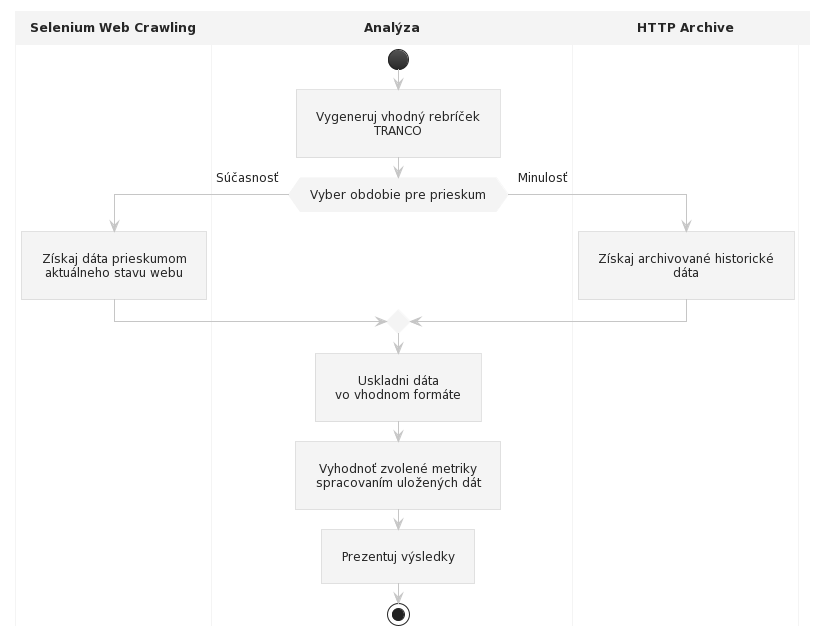
\includegraphics[scale=0.48]{obrazky-figures/analysis-activity-diagram.png}    
 % 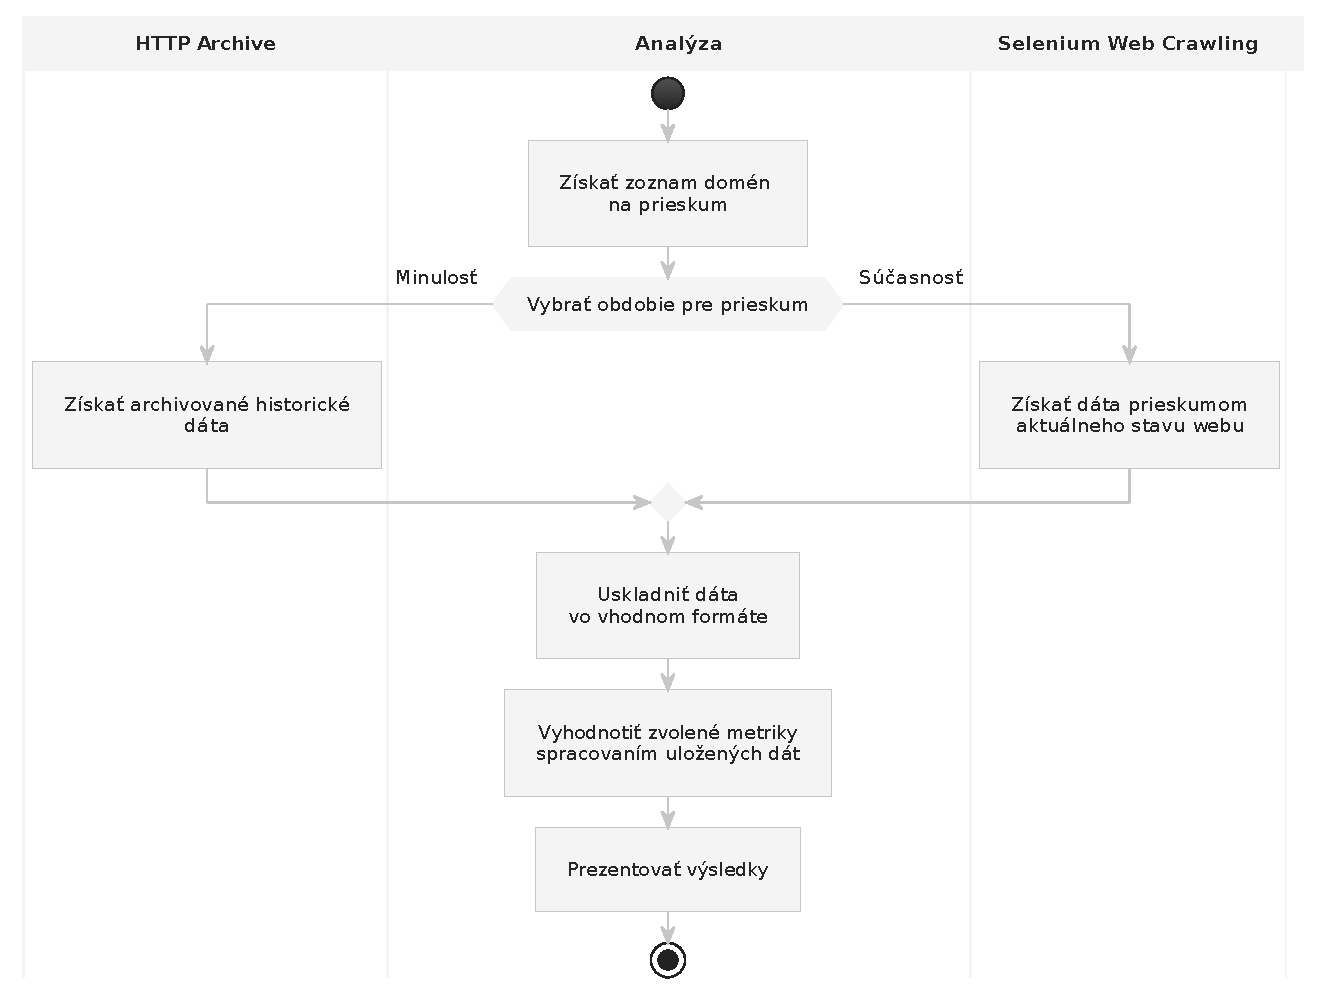
\includegraphics[scale=0.65]{obrazky-figures/analysis-activity-diagram-hd.pdf}    
 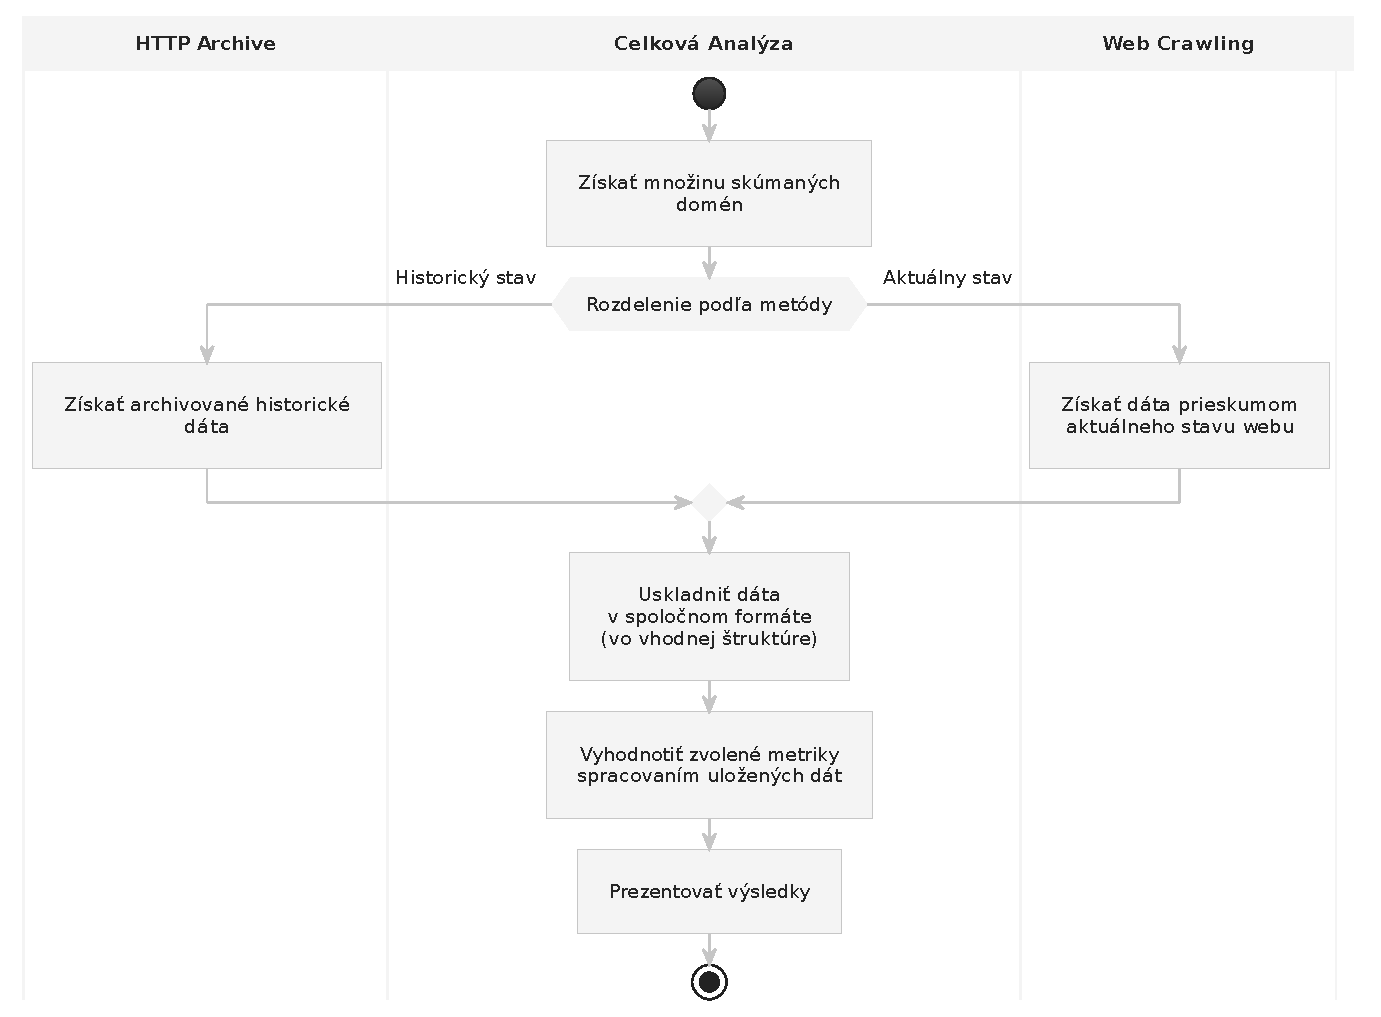
\includegraphics[scale=0.65]{obrazky-figures/analysis-activity-diagram-revised.pdf}    
 \caption{\centering Diagram aktivít analýzy.}
 \label{img:analysis-activity-diagram}
\end{center}
\end{figure}


% \noindent V tejto kapitole popisujem návrh na vypracovanie analýzy nasadenia a využívania technológie NEL.
% Najskôr uvediem, aké poznatky boli zistené v už existujúcich prácach. Ďalej predstavujem rozsah a rozdelenie vlastnej analýzy na postupnosť potrebných krokov k jej vykonaniu.
% Potom prechádzam k spôsobom, akými jednotlivé časti navrhujem vypracovať.

% \section{Poznatky z existujúcej analýzy}
% \label{praca-veduceho}
% \label{skript}

% Existuje predošlá analýza zameraná na technológiu NEL \cite{nel-http-archive}. 
% Je zameraná na získanie metrík ako celkovú využívanosť NEL na sade skúmaných domén, aké NEL kolektory dané domény používajú a v akých konfiguráciach sa nasadené NEL vyskytuje.
% Časové obdobie, za ktoré bola analýza zhotovená, tvorili februárové mesiace každého roku od 2018 do 2023. 
% Za toto obdobie sa podarilo zistiť, že počiatočné využitie NEL bolo 0\% a do februára roku 2023 stúplo na 11.73\% skúmaných domén.
% Toto percento predstavuje z celkového zoznamu skúmaných domén 2,247,233 jedinečných domén.

% \begin{figure}[!htb]
% \begin{center}
%     % 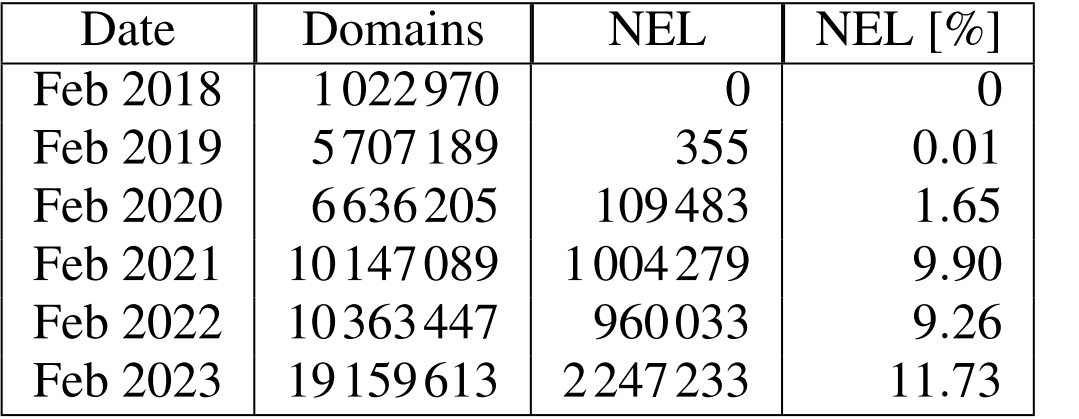
\includegraphics[width=0.5\linewidth]{obrazky-figures/polcak-analysis.png}
%     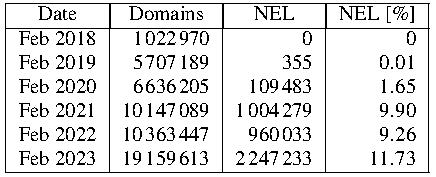
\includegraphics[width=0.55\linewidth]{obrazky-figures/polcak-analysis-hd.pdf}
%     \caption{\centering Využitie NEL na skúmaných doménach v analýze vypracovanej vo vedeckom článku Ing. Libora Polčáka Ph.D. a Ing. Kamila Jeřábka \cite{nel-http-archive}.}
%     \label{fig:polcak-analysis}
% \end{center}
% \end{figure}

% Je dôležité poznamenať, že sa táto analýza pracovala iba s domovskými stránkami pre každú skúmanú doménu.
% To znamená, že bol pre každú cieľovú doménu preskúmaný práve jeden zdroj na nej dostupný.
% Keďže bol v rámci práce použitý projekt HTTP Archive ako zdroj dát, toto rozhodnutie mohlo zapríčiniť to, že ním využívaná služba Google Cloud je spoplatnená (viď sekciu \ref{big-query}). 
% Je pravdepodobné, že autori nemali prostriedky pre financovanie spracovania takého veľkého objemu dát, ktorý predstavuje skúmané obdobie šiestich rokov.
% Vo svojej práci usúdili, že vzhľadom na túto limitáciu je nutné vypracovať podrobnejšiu analýzu, doplnenú o dáta získané alternatívnym spôsobom \cite{nel-http-archive}.
% Práve z toho dôvodu je nutné v mojej analýze okrem použitia HTTP Archive navrhnúť aj iný spôsob skúmania stavu využitia technológie NEL.


% \section{Vlastná analýza}

% Mojim cieľom je podrobne analyzovať využívanie technológie NEL na webe. 
% Podľa prieskumu možných zdrojov dát pre analýzu z predošlej kapitoly možno vypracovať vlastnú analýzu v nasledujúcich krokoch:
% \begin{enumerate}
%     \item vybrať domény, ktoré budem skúmať,
%     \item získať záznamy HTTP odpovedí z web stránok na daných doménach,
%     \item zo získaných záznamov vyhodnotiť využívanosť NEL v podobe rôznych metrík
%     \item a nakoniec vhodne prezentovať vyhodnotené metriky ako výsledky.
% \end{enumerate}

% \begin{figure}[!htb]
% \begin{center}
%  % 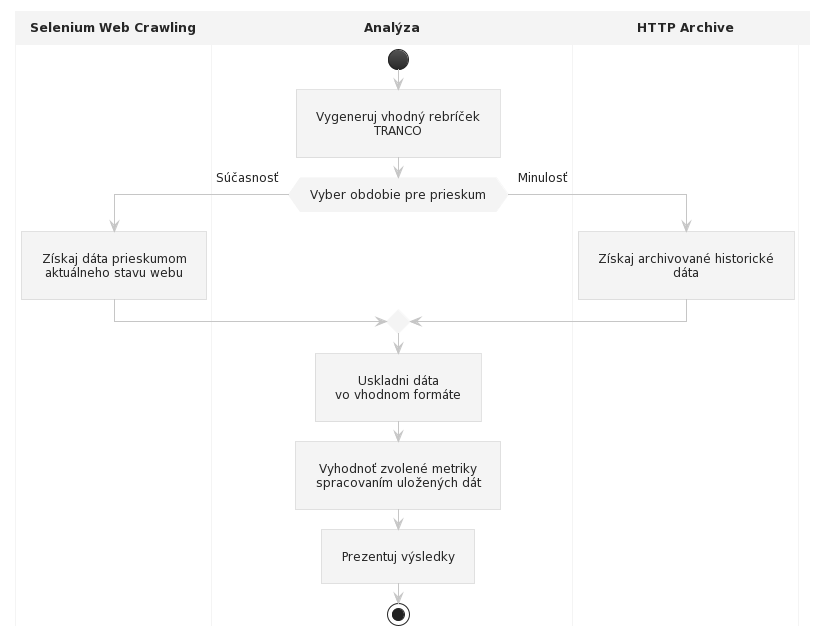
\includegraphics[scale=0.48]{obrazky-figures/analysis-activity-diagram.png}    
%  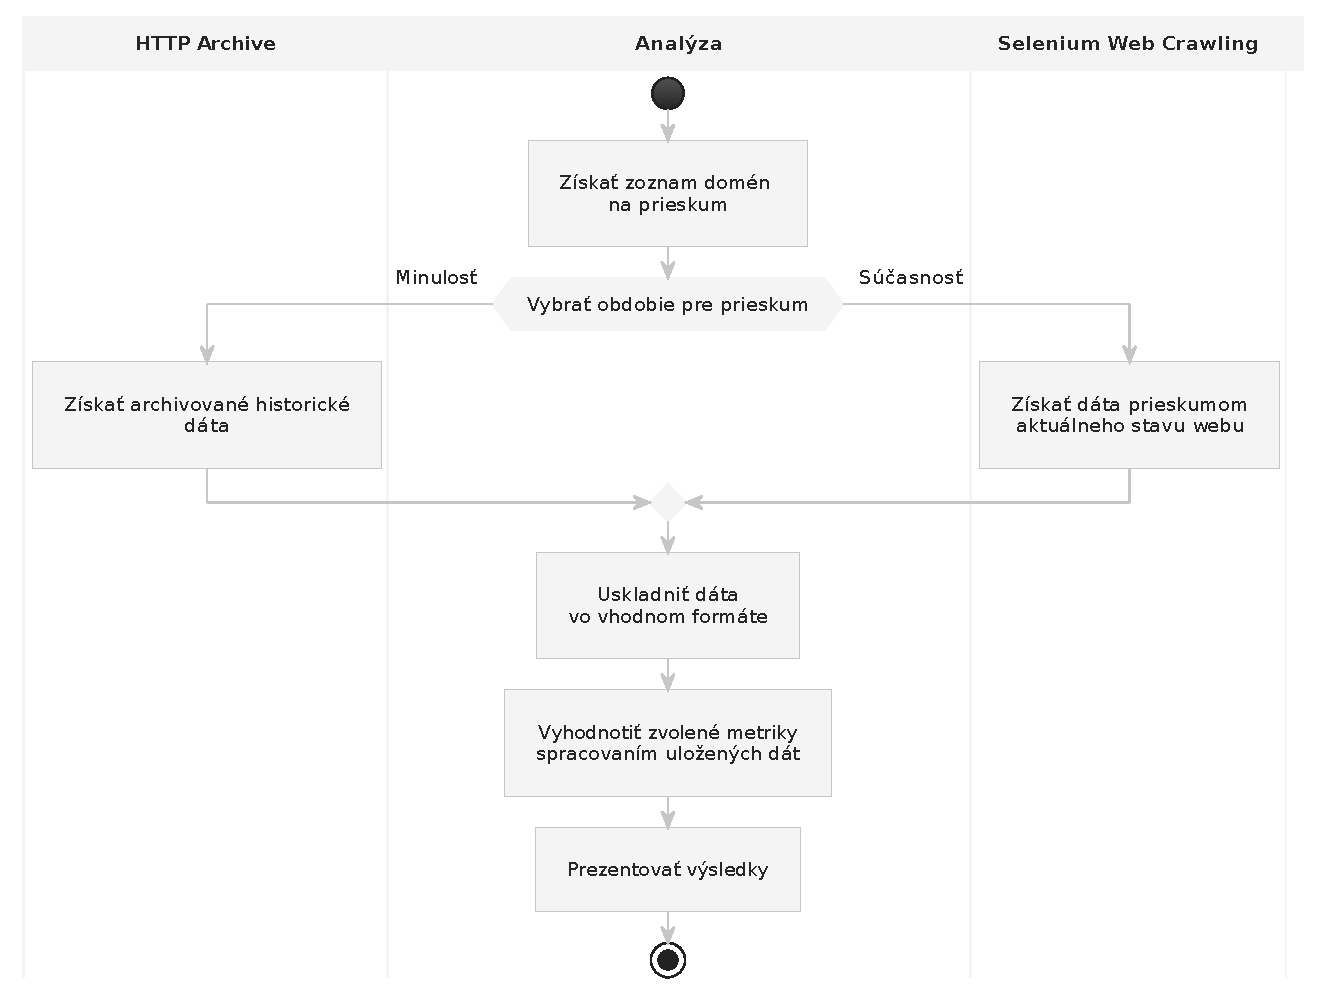
\includegraphics[scale=0.65]{obrazky-figures/analysis-activity-diagram-hd.pdf}    
%  \caption{\centering Diagram možných aktivít pre čiastkové úlohy vlastnej analýzy.}
%  \label{img:analysis-activity-diagram}
% \end{center}
% \end{figure}


% \subsubsection{Skúmané domény}

% V záležitosti výberu skúmaných domén som uznal za vhodné vybrať domény z dát projektu HTTP Archive.
% Viackrát spomínaný rebríček TRANCO som sa rozhodol nevyužiť ako hlavný zoznam domén na skúmanie primárne preto, že oproti HTTP Archive ponúka značne menej domén.
% Z pokusov generovania rebríčkov TRANCO som zistil, že jeho veľkosť sa približuje k maximu okolo 4 miliónov domén.
% HTTP Archive nahromaždené mesačné dáta však obsahujú viac jedinečných domén už od prvého dňa, za ktorý je možné vygenerovať rebríček TRANCO.
% Pri celkovej analýze ale tento rebríček môže byť v prípade potreby stále užitočný pre zameranie sa na tie najpopulárnejšie domény z celkovej skúmanej množiny.

% \subsubsection{Získavanie potrebných dát}

% Samotné dáta, ktoré ako vstup pre analýzu potrebujem sú záznamy HTTP odpovedí z webových stránok na skúmaných doménach.
% K takýmto dátam poskytovaným projektom HTTP Archive mám prístup cez rozhranie Google Cloud.
% Keďže tieto dáta boli analyzované iba pre februárové mesiace každého skúmaného roka,
% pokúsim sa preskúmať celý rozsah skúmaného obdobia, a to od dátumu verejného publikovania špecifikácie NEL --- 25. septembra 2018 --- až po najaktuálnejšie dáta dostupné z HTTP Archive.
% Podľa zistení v práci spomínanej v predošlej sekcií je pri tom dôležité pokúsiť sa optimalizovať spôsob získavania dát z ich úložiska.
% Optimalizácia sa týka minimalizovania využitia finančných zdrojov potrebných na získanie žiadaných dát.

% Pre prieskum aktuálneho stavu som sa rozhodol navrhnúť a implementovať vlastný program na prechádzanie webu -- web crawler.
% Jeho úlohou bude prechádzať web stránky dostupné na skúmaných doménach a ukladať záznamy o nájdených NEL HTTP hlavičkách.
% Vzhľadom na to, že v tomto prípade ide o aktuálny stav webu, vyberiem ako vstupné domény tie, ktoré obsahuje dataset z posledného mesiaca HTTP Archive.

% \subsubsection{Spracovanie dát a výsledky}

% Po získaní historických a aktuálnych dát nasleduje hlavná časť práce, a to vyhodnotenie výsledkov.
% Využitím nadobudnutých záznamov HTTP odpovedí zo skúmaných domén sa zameriam na výpočet niekoľkých metrík:
% \begin{itemize}
%     \item počet domén, ktoré NEL využívajú,
%     \item NEL kolektory, ktoré sa využívajú, ich počet a najvyužívanejšie z nich,
%     \item konfigurácie, v ktorých sa vyskytuje využívaný NEL,
%     \item pomer monitorovaných zdrojov k všetkým zdrojom dostupných na danej doméne,
%     \item typy monitorovaných zdrojov,
%     \item a nesprávne nasadenie NEL.
% \end{itemize}

% \noindent Po spracovaní dát a vyhodnotení zvolených metrík budem výsledky prezentovať zvlášť pre historické a pre aktuálne dáta.  